\chapter{Background Theory}

\label{ch:background}

\section{Modelling Infectious Disease Dynamics}
Throughout history, infectious diseases can consistently be cited as one of the leading causes of death across the world. Whilst many such diseases may be endemic in a population,  a large proportion  of diseases may outbreak as epidemics. That is, a disease may arise in a community, region or even worldwide in excess of normal levels following a particular outbreak. In an age of increasing urbanisation, global connectivity and a larger immuno-compromised population, monitoring and controlling the spread of epidemics is absolutely paramount.\cite{computational} Recent events such as the 2009 flu pandemic highlight the incredible need for a solid understanding of the underlying mechanisms of such diseases. This section will discuss the history and current standards in epidemiology.

A general understanding of infectious disease behaviour can be seen as early as the 8th century A.D., when the Indians and Chinese used a rudamentary form of vaccination known as variolation to control smallpox.\cite{variolation} Even earlier than this, Hippocrates (c. 460-c. 370 BC) was amongst the first to propose that disease spread could be explained rationally through human behaviour and environmental factors.\cite{hippo} Unfortunately, the understanding of infectious disease dynamics appeared to regress until the 17th century when the collection of the first public health statistics allowed for a more scientific approach. 

One of the first predictive mathematical models was by Bernoulli in 1760, who used mathematical techniques to establish that variolation for smallbox could help increase the life expectancy in the French population.\cite{brauer} Similarly, another systematic study of disease dynamics took place in 1854 by John Snow, who identified a single water pump in London as the likely source of a Cholera epidemic.\cite{snow} However, it was the early 1900s in which the most fundamental advances in mathematical epidemiology were made. Firstly by Ross in 1911, who used a spatial model to describe the spread of malaria due to mosquitoes.\cite{snow} This study was the first to demonstrate that infectious diseases could be controlled by reducing the population of infected individuals below a certain threshold. The next and arguably most central breakthrough was then made by Kermack and McKendrick in 1927, who proposed the use of ordinary differential equations (ODEs).\cite{kermack} ODEs represented the first deterministic, general epidemic model to describe mass action. The general idea behind ODE models in the context of epidemiology is that individuals in a given population are members of various compartments depending on their relationship to the infection (eg. infected, recovered), and individuals switch between compartments as described by these ODEs.

The most basic form of the model prosed by Kermack and McKendrick's ODEs is the Susceptible-Infected-Recovered (SIR) model. Given a population of size N, individuals are divided into three states or compartments: 

\begin{enumerate}
	\item Individuals that are susceptible to the infection, denoted by $S(t)$
	\item Individuals that are infected with the disease and are therefore capable of infecting others, denoted by $I(t)$
	\item Individuals that have been removed from the population or recovered, denoted by $R(t)$. 
\end{enumerate}

Individuals move between compartments in the following order:
\begin{equation*}
S \Longrightarrow I \Longrightarrow R
\end{equation*}
Simply, individuals start off as being free of the disease, but susceptible to infection. Individuals are then infected with the disease and begin to display symptoms, thereby becoming infectious themselves. After a certain period of time, individuals are no longer infectious as they recover and become immune to the disease. In this model, the population size is assumed to be fixed such that:

\begin{figure}[ht!]
\centering
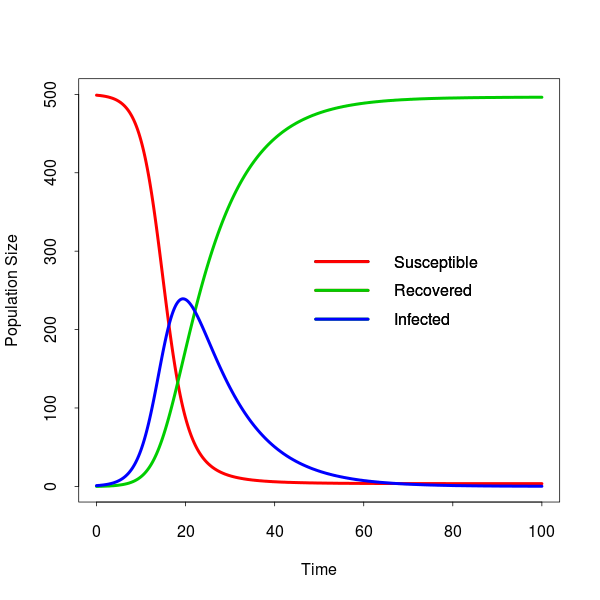
\includegraphics[width=120mm]{Rplot.png}
\caption{Generic example of the classic SIR model demonstrating the change in population size for each compartment as the epidemic unfolds}
\label{sir}
\end{figure}

\begin{equation*}
N = S(t) + I(t) + R(t)
\end{equation*}

The way in which individuals individuals move between these compartments are described by the following set of ODEs:
\begin{equation*}
	\begin{split}
	&\frac{dS}{dt} = -\beta IS, \\
	&\frac{dI}{dt} = \beta IS - \gamma I, \\
	&\frac{dR}{dt} = \gamma I
	\end{split}
\end{equation*}

The dynamics of these ODEs are influenced by two key parameters: the contact rate, $\beta$, and the recovery rate, $\gamma$. $\beta$ describes the probability of an infected person coming into contact with any susceptible person per unit time, whereas $\gamma$ describes the rate at which an individual recovers from the disease. When $\beta$ is large, the contact rate between individuals is high, and the disease spreads rapidly. Similarly, when $\gamma$ is large, then individuals recover rapidly and move to the recovered compartment quickly. Note that these parameters make global assumptions about the population, in that all individuals have an equal chance of interacting, and all individuals recover at the same rate. Infected individuals therefore come into contact with $\beta$$N$ individuals per unit time. Only susceptible individuals may become infected, and the number of new infections per unit time is therefore $\beta$$N(S/N)$, resulting in a new infection rate of $\beta$$N(S/N)I = $$\beta$$SI$. Finally, as individuals recover with rate $\gamma$, they are removed from the infected compartment and enter the recovered department with rate $\gamma I$.

Considering these parameters allow for useful insights into the dynamics of a given disease: a disease with a high $\beta$ and lower $\gamma$ will obviously spread more than one with a lower contact rate and higher recovery rate. With this in mind, we can make the intuitive leap to conclude that an infection will either: spread as an epidemic when each individual is causing more than one secondary infection; remain endemic in a population when each individual causes exactly one further infection before recovering; will die out when each individual causes less than one secondary infection before recovering. This idea is formalised by the concept of a \emph{basic reproductive number}, $R_0$ (not to be confused with $R(0)$, which denotes the initial size of the recovered population!). $R_0$ denotes the number of secondary infections caused by a single infected individual when introduced into an initial susceptible population, $S(0)$. As this infected individual will come into contact with $\beta N$ individuals per unit time over a period of $1/$$\gamma$ (the mean infectious period), the reproductive number will be given as the number of secondary infections per unit time multiplied by the amount of time that an individual can infect others:\cite{anderson, diekmann}

\begin{equation*}
R_0 = (\beta N)/\gamma
\end{equation*}

$R_0$ describes the number of secondary infections resulting from one individual in a completely susceptible population; however, this rate will obviously decrease as the proportion of susceptible individuals in the population decreases. Rather than considering the initial reproductive number, it is often more useful to consider the effective reproduction number, $R_n$ . In simplest terms, $R_n = R_0 \times s$, where $s$ is the proportion of the population that is susceptible ($S(t)/N$).

As an aside, it should be noted that calculating $R_0$ is a crucial stage in understanding how a disease will spread. A high $R_0$ (eg. malaria) means that the disease will spread rapidly, with each individual causing a high number of secondary infections, whereas a low $R0$ (eg. monkeypox) means that a disease will spread slowly.\cite{vynnycky} As discussed above, an $R_0$ greater than 1 is necessary for an epidemic to take hold. Even at an early stage of an epidemic, $R_0$ can be estimated based on the growth rate of an epidemic, as was the case during the 2003 SARS virus.\cite{sars} Therefore, decreasing the proportion of sucseptible individuals below a certain level (ie. through vaccination) will result in an effective reproduction number of less than 1, preventing the epidemic from taking hold. This critical threshold is defined as the \emph{herd immunity threshold}, and provides a crude but often effective target for immunization programmes:\cite{cockman}

\begin{equation*}
HIT = 1 - \frac{1}{R_0} = \frac{R_0 -1}{R_0}
\end{equation*}

The model shown above describes three compartments, however there are a number of extensions to this model where different compartments and interactions might be appropriate. For example, an "exposed" compartment might be added which encompasses individuals that have been exposed to the disease, but are not yet infectious. Such a model is known as the SEIR model. As well as additional compartments, the transitions between these compartments might be varied. For example, in cases where immunity is only transient, individuals might be able to re-enter the susceptible compartment following recovery (the SIRS model). Choosing the model structure is dependent on the nature of the disease and population under consideration. For example, using an SIS (infected individuals return to the susceptible state) to model HIV, or an MSIR model (initial maternal-derived immunity) in the case of measles.\cite{vynnycky} 

It should be noted that there are further considerations to take when modelling real epidemics. For example, the inclusion of birth and death rate, seasonal dynamics, stochasticity and age-dependent interactions.\cite{vynnycky} However, the basic principles discussed above are sufficient to begin considering how we might model the spread of other epidemic processes. 

With the solid theoretical basis described above, advanced mathematical and computational models are becoming increasingly central to making public health decisions. One recent application of mathematical models in epidemiology was to describe and predict the dynamics of an epidemic in real time.\cite{kerkhove} A study by Tizzoni et al. used a Monte Carlo Maximum Likelihood (MCML)-based approach on historical data from the 2009 flu pandemic to develop a global stochastic simulation model, referred to as GLEAM, to obtain basic model parameters.\cite{gleam, gleam2} (Note that this project will aim to similar methodologies to fit epidemic models in real time, and a brief overview of maximum-likelihood estimation and least squares estimation is provided in Box 1). Tizzoni et al. used GLEAM to estimate the seasonal transmission ability of the 2009 H1N1 pandemic, generating forecasts for the activity peaks in the northern hemisphere. The robustness of this stochastic forecast was also explored as a function of data completeness by fitting the model using only partial data.\cite{tizzoni} 

Tizzoni et al. showed that the GLEAM model was in good agreement with
the actual 2009 epidemic data, even when only partial data was used
(for example, pre-exposure immunity and adherence to vaccination
campaigns. However, a key feature of the model is that it accounts for
the way in which  populations interact and connect, and it was shown
that model accuracy was reduced considerably when using only a partial
dataset for population mobility. The GLEAM model uses three layers: a
population layer (a grid representing the population of the world); a
mobility layer (using real flight data to represent travel between
cells in the grid); and an epidemic model (consisting of susceptible,
latent, symptomatic infectious able to travel, symptomatic infectious
unable to trabel, asymptomatic infectious and permanently covered
compartments). Indeed, consideration of multiple networks layers in
epidemic modelling is a growing area of consideration for real
infectious diseases, as it alows for the consideration of more
realistic population dynamics.\cite{gefm} \\\\

\newpage
\begin{framed}
{\begin{center}{\bf Box 1}\end{center}}
To fit model parameters in real time, we consider two methods to fit a continuous-time model to a given set of data: least squares and Maximum Likelihood Estimation (MLE).

{\bf Least squares} is the simpler of the two approaches, and assumes that the only source of variability in the data is measurement error (which is distributed symmetrically with a constant variance eg. Gaussian). By estimating the "least squares" for a set of parameters, we aim to find the set of parameters that minimises the sum of the squares of the errors (ie. the difference between an observed value and the fitted value). 

More formally, given a simple data set of $n$ points of the form $(x_i, y_i)$, we aim to minimise the following formula:
\begin{equation*}
S = \sum\limits_{i=1}^n r_{i}^2
\end{equation*}

Where $r_i$ is the residual for each point, given by the difference between the actual value of the dependent variable and the variable fitted by the model: $r_i = y_i - f(x_i, \beta)$

In the context of our SIR model, we aim to find the $\beta$ and $\gamma$ values that provide the best fitting SIR model for a given epidemic dataset (we will use the Nelder-Mead algorithm with \emph{R}).\cite{marily2013}

{\begin{center} 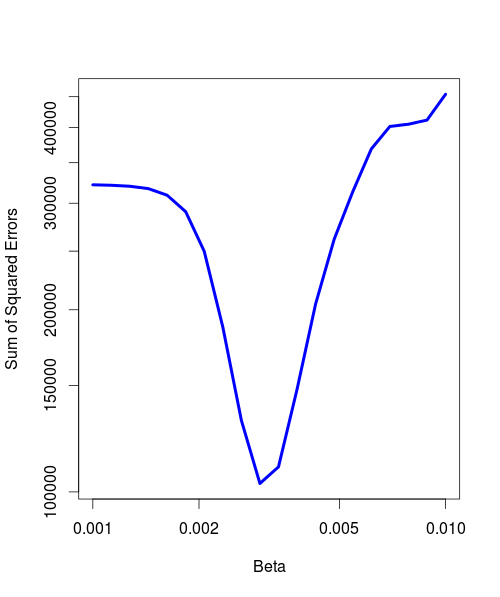
\includegraphics[width=100mm]{sse.png}\end{center}}

Shown above is an example sum of squared errors (SSE) plot demonstrating how a particular value for $\beta$ minimises the SSE to a given dataset at around 0.003. This plot was created using a test flu dataset. Note that this plot assumes a $\gamma$ value of 1, though multiple parameters may be optimised simultaneously using R's \emph{optim} (Nelder-Mead) function.

{\bf Maximum-likelihood estimation} (MLE) is the method of estimating the parameters of a statistical model based on a given hypothesis and a set of data that has occured. This method essentially selects the set of values for the model parameters that maximise the likelihood function:
\begin{equation*}
	\mathcal{L} (\theta | x) = P(x | \theta)
\end{equation*}
In other words, we aim to find the set of parameters that  provide a model fit would be most likely to produce our given data. As above, we aim to find the set of parameters, $\beta$ and $\gamma$ that maximise this likelihood function. Specifically, we calculate the negative log-likelihood of the data given some combination of parameters. Methods using MLE are very common when fitting epidemic models in real time.\cite{white, hall, nishiura}
{\begin{center} 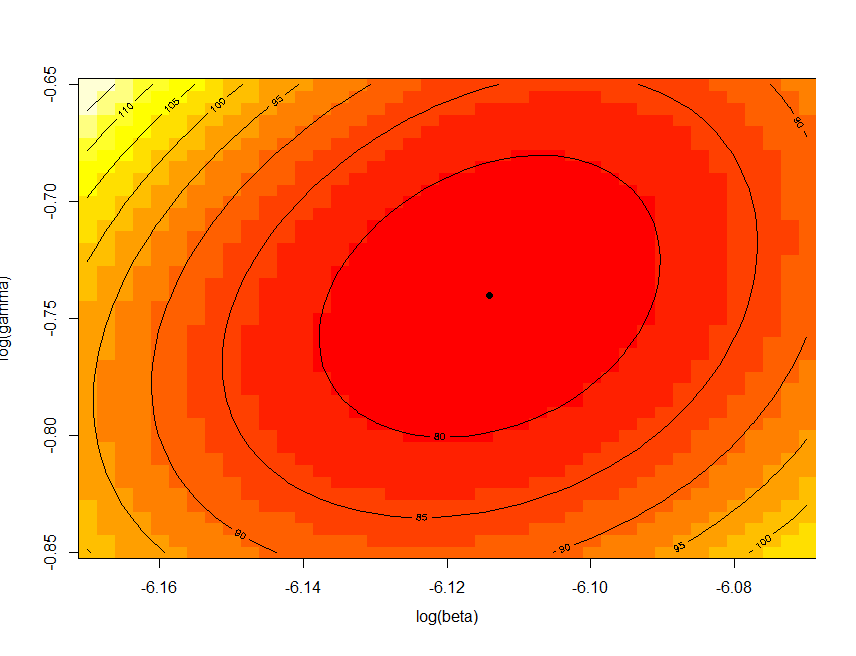
\includegraphics[width=140mm]{logmle.png}\end{center}}
The graph above depicts the two-dimensional parameter space (the likelihood surface) for beta and gamma when fit to a set of epidemic data. Note that we use log values to avoid underflow/overflow.  Each point represents a separate fit to the data, and the height of the surface shows the negative log-likelihood of that parameter combination. In this particular example, we find that a log(beta) value of ~-6.11 and a log(gamma) value of ~-0.74 provide the best fit. We can also show the confidence intervals for each parameter in the form of a likelihood profile, as shown below.

{\begin{center} 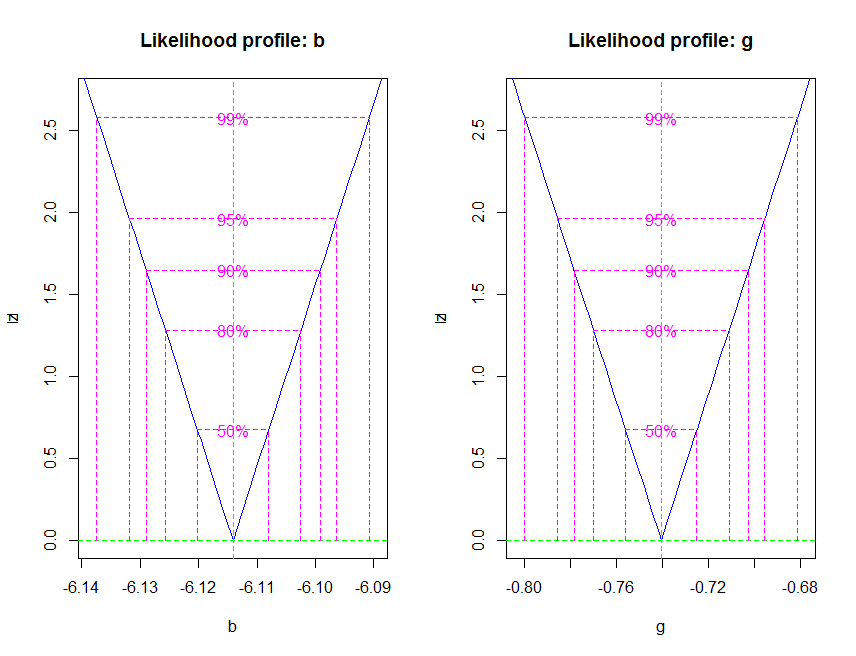
\includegraphics[width=140mm]{mle.png}\end{center}}

\end{framed}

\section{Epidemic Phenomena on the Internet}
A more recent application of epidemic modelling methods is to the spread of information and trends. In particular, the continual development of the internet has opened up a vast area of research into the dynamics of social networks, viral marketing and computer security. It is quite easy to see the analogy between the spread of an online trend to the spread of an infectious disease: individuals have either been exposed to the trend or not; may be actively spreading the trend; or may have lost interest in the trend. The relatively recent surge of interest in online social networks and rapidly rising occurence of viral phenomena has brought with it an interest in understanding and modelling these trends. In this section, we will briefly discuss the history of epidemiology-based analyses of information dissemination and the resulting application of classical epidemiology to online phenomena.

The first application of epidemiology in a social context was made by Goffman and Newill in 1964 who directed attention to the analogy between the spreading of an infectious disease and the dissemination of information.\cite{goffman} This was closely followed by Daley and Kendal, who examined the spreading of rumours using mathematical epidemiology.\cite{goffman} As in Kermack and McKendrick's SIR model, Daley and Kendal used three compartments to describe their population: those individuals that had not heard the rumour, those that were actively spreading the rumour and those that were no longer spreading the rumour. The way in which these compartments interacted was described by parameters indicating those that heard the rumour and those that lost interest or `forgot' the rumour, corresponding to $\beta$ and $\gamma$. Daley and Kendal found that the fit was somewhat limited by the difference in behaviours of a rumour and an infectious disease. Specifically, the way in which individuals "lost interest"  in the rumour was not comparable to recovery from an infectious disease. Although not a perfect fit, Daley and Kendal's study did highlight the potential application of mathematical epidemiology in a social context.

More recently, the ever increasing relevance of the internet to modern day life has resulted in more studies being undertaken to model and predict the spread of trends and information on the internet. Bauckhage et al. present one such study, investigating the application of statistical models in describing the spread of internet memes.\cite{meme} That is, viral catch phrases, images or videos that spread through instant messaging, blogs, forums and social networking sites. Bauckhage et al. use \emph{Google Trends} data as an indicator of search frequency and therefore interest in the internet population. Classiying these as `fads', Bauckhage et al. go on to fit established statistical distributions to over 200 meme related time series compared to a fitted Log-Normal model. Using a multinomial maximum likelihood fit, the authors find that the Weibull, Gompertz and Frechet distributions all provided a better model of general trends for meme related search activity, suggesting that growth dynamics cannot be attributed to chance. The authors conclude that these dynamics can be described as a `hype cycle', encompassing a period of rapid uptake followed by a gradual loss of appeal. Although Bauckhage et al. did not use epidemic modelling, they demonstrated that mathematical modelling could be effectively used to describe online trend dynamics.

\begin{figure}[ht!]
\centering
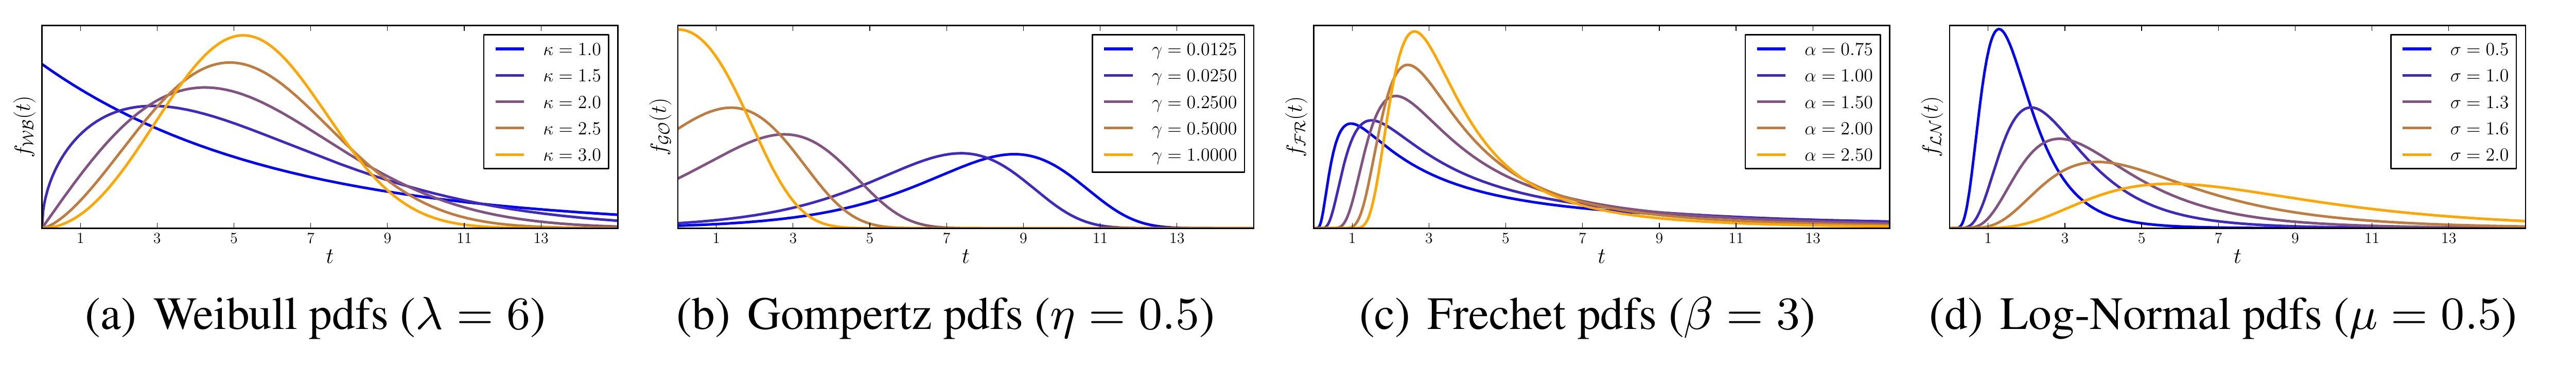
\includegraphics[width=160mm]{statsdist.png}
\caption{Examples of the statistical distributions considered in Bauckhage et al.\cite{meme}}
\label{sir}
\end{figure}

The study by Bauckhage et al. demonstrates the applicability of mathematical modelling to the dynamics of internet memes, however research has also been undertaken to describe the spread of internet `celebrities'. Tweedle and Smith undertook one such study, investigating the usefulness of SIR modelling in describing the spread of popularity of the music artist, Justin Bieber.\cite{bieber} Tweedle and Smith demonstrated that an SIR model could be fit to \emph{Google Trends} search data relatively well. Furthermore, the study investigated how `media effects' might impact epidemic spread (for example, an album release or television appearance). It was found that the inclusion of media effects improved the usefulness of the model in describing the search trend data. Although a fairly `tongue in cheek' study, Tweedle and Smith demonstrated that SIR modelling could be successfully used to describe the spread of online popularity, particularly when additional media effects are considered.

A recent study by Nika et al. showed the potential for epidemiology to explain and predict outbreaks of internet-based information spreading, with the novelty that the size of the initial susceptible population was assumed to be unknown.\cite{marily2013} The aim of this study was to fit SIR and SEIR models to celebrity outbreaks on the internet in real time, improving model fit as the epidemic progresses. Using the Nelder-Mead algorithm with a least-squares-based objective function to fit SIR and SEIR models in real time (see Box 1), Nika et al. were able to demonstrate real time model fitting with unknown initial parameters. The authors validate their approach on synthetic epidemic data, a historical influenza epidemic and BitTorrent and YouTube video views. Both the SIR and SEIR models fit the synthetic and historical data well, and showed good predictive power. However, whilse the models were fit to the internet-based data with some success, the authors acknowledge limitations in their methodology, such as the generation of confidence intervals without due regard for parameter uncertainty. This study demonstrates a promising framework for fitting parameters to data in real time, though highlights the limitations of classic SIR modelling in its basic form.

One recent study using similar methodology that recently received public interest was by Cannarella and Spechler, who investigated the use of SIR modelling in describing public interest in OSNs, namely MySpace and Facebook.\cite{cannarella} Cannarella and Spechler used an adapted SIR model that modified the dynamics of the recovering population such that contact between recovered and infected individuals was required for recovery.  That is, individuals would only stop using the OSN if they came into contact with someone who had already stopped using it. The authors named this adaptation the `irSIR' model. As in the above studies, Cannarella and Spechler used \emph{Google Trends} search data as a proxy for service usage. Similar to Nika et al., the authors used the Nelder-Mean algorithm to find a best fit curve based on sum of squared error, also assuming that all initial parameters, including population size are unknown. The study found that in the case of MySpace, whilst the basic SIR model did not fit particularly well, the modified irSIR model provided a good fit to the adoption and abandonment phases of the OSN. When applied to the ongoing OSN, Facebook, the authors found that Facebook had reached peak popularity in 2012 and was in the early stages of abandonment, predicting that the OSN would reach 20\% of its maximum size by the end of 2014. The authors do concede that there exists an infinite range of possible slower declining solutions. 

Facebook posted a rebuttal to the study, using similar methodology to show that Princeton would cease to exists by 2021 based on Google search results.\cite{facebook} Although not a formal, peer revewed study, Facebook's rebuttal did highlight some shortcomings with the methodology employed by Cannarella and Spechler. Namely the assumption that Google searches were an indicator of usage, and also the flawed assumption that Facebook would not `evolve' to keep users. These studies highlight the importance of making valid assumptions and using appropriate data when attempting to study a rapidly evolving area such as OSNs.

With huge implications for marketing and commercial success, Interest in viral phenomena has become an area of particular interest outside of the academic community. As a result, commercial circles have also taken an interest in attempting to understand the spread of online trends. A review posted by the global strategic insight agency, \emph{Facegroup}, inadvertantly touched upon the application of SIR modelling in explaining the spread of viral videos.\cite{facegroup} The main conclusion that  \emph{Facegroup} came to was that there is no single model of virality. Rather, different types of viral videos could be spread in different ways, proposing `spike' and a `growth' types depending on their spreading pattern. In the `spike' case, videos tend to peak early and drastically drop in views within a week. In the latter case, videos achieve their peak views after a few days and decline slowly, interrupted by secondary peaks of interest. 
\newpage
\begin{figure}[ht!]
\centering
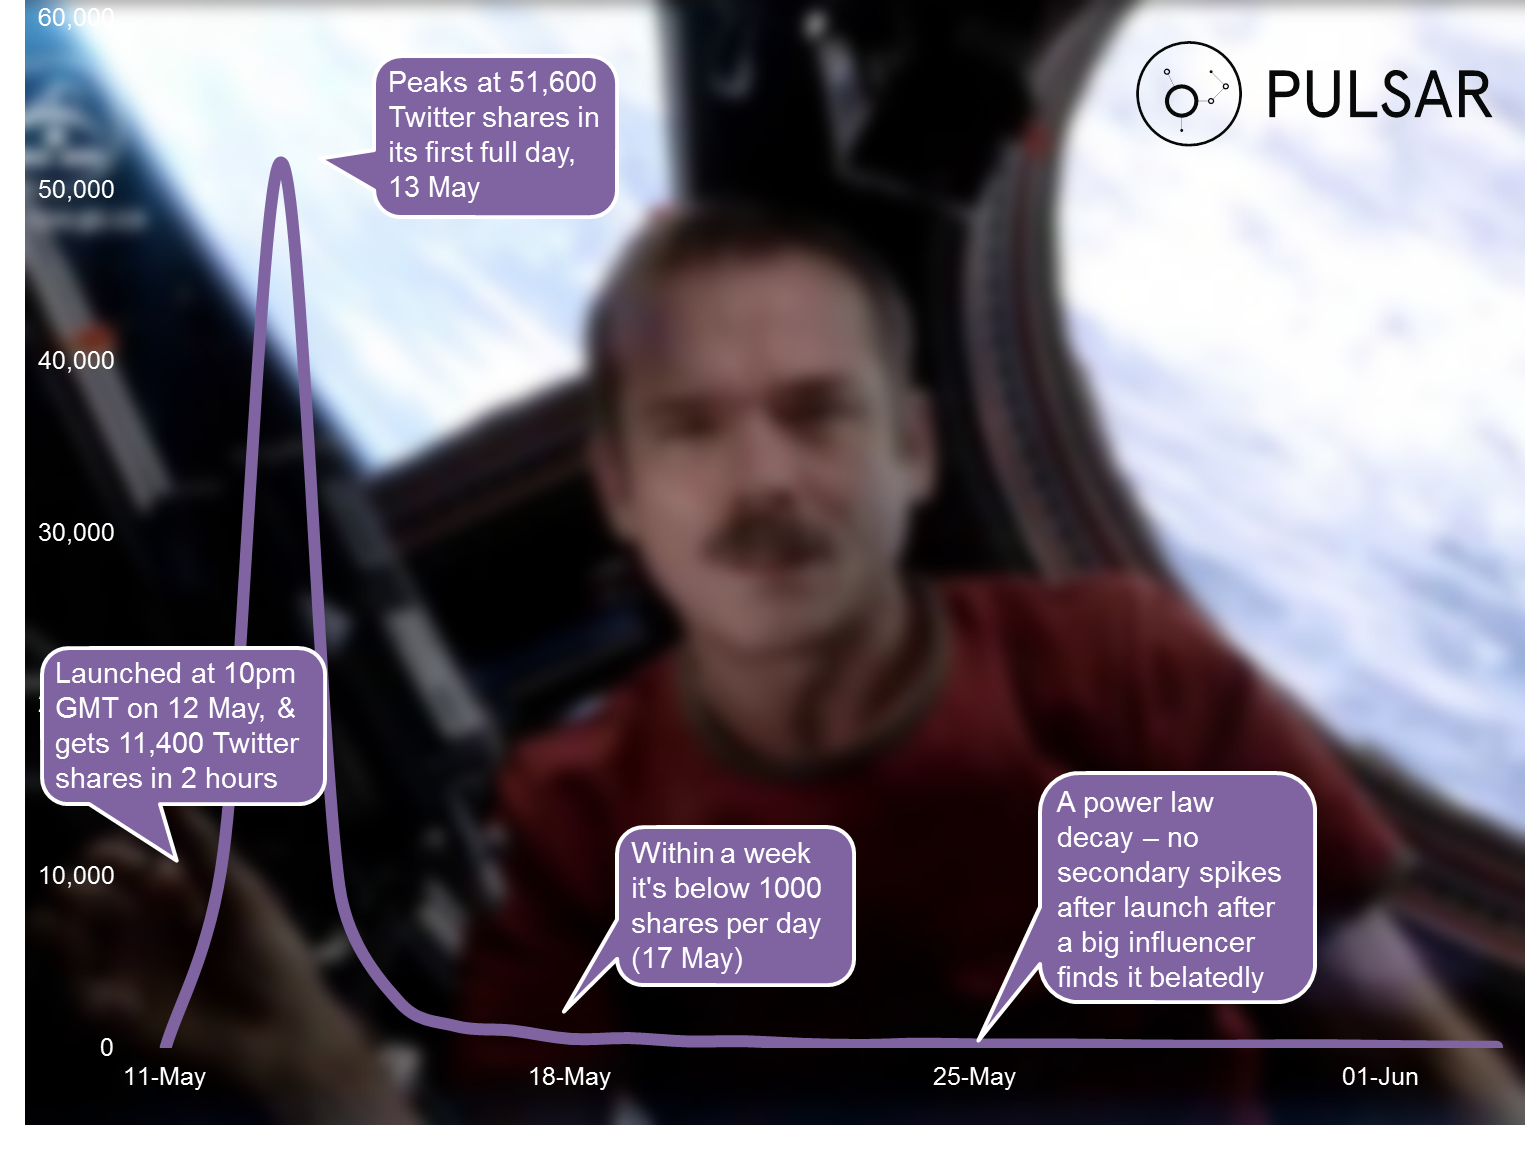
\includegraphics[width=120mm]{hatfield.png}
\caption{Graph \emph{Facegroup} depicting the uptake of the "Commander Hadfield" YouTube video, demonstrating the "growth" model as proposed by \emph{Facegroup}.\cite{facegroup}}
\label{sir}
\end{figure}

\begin{figure}[ht!]
\centering
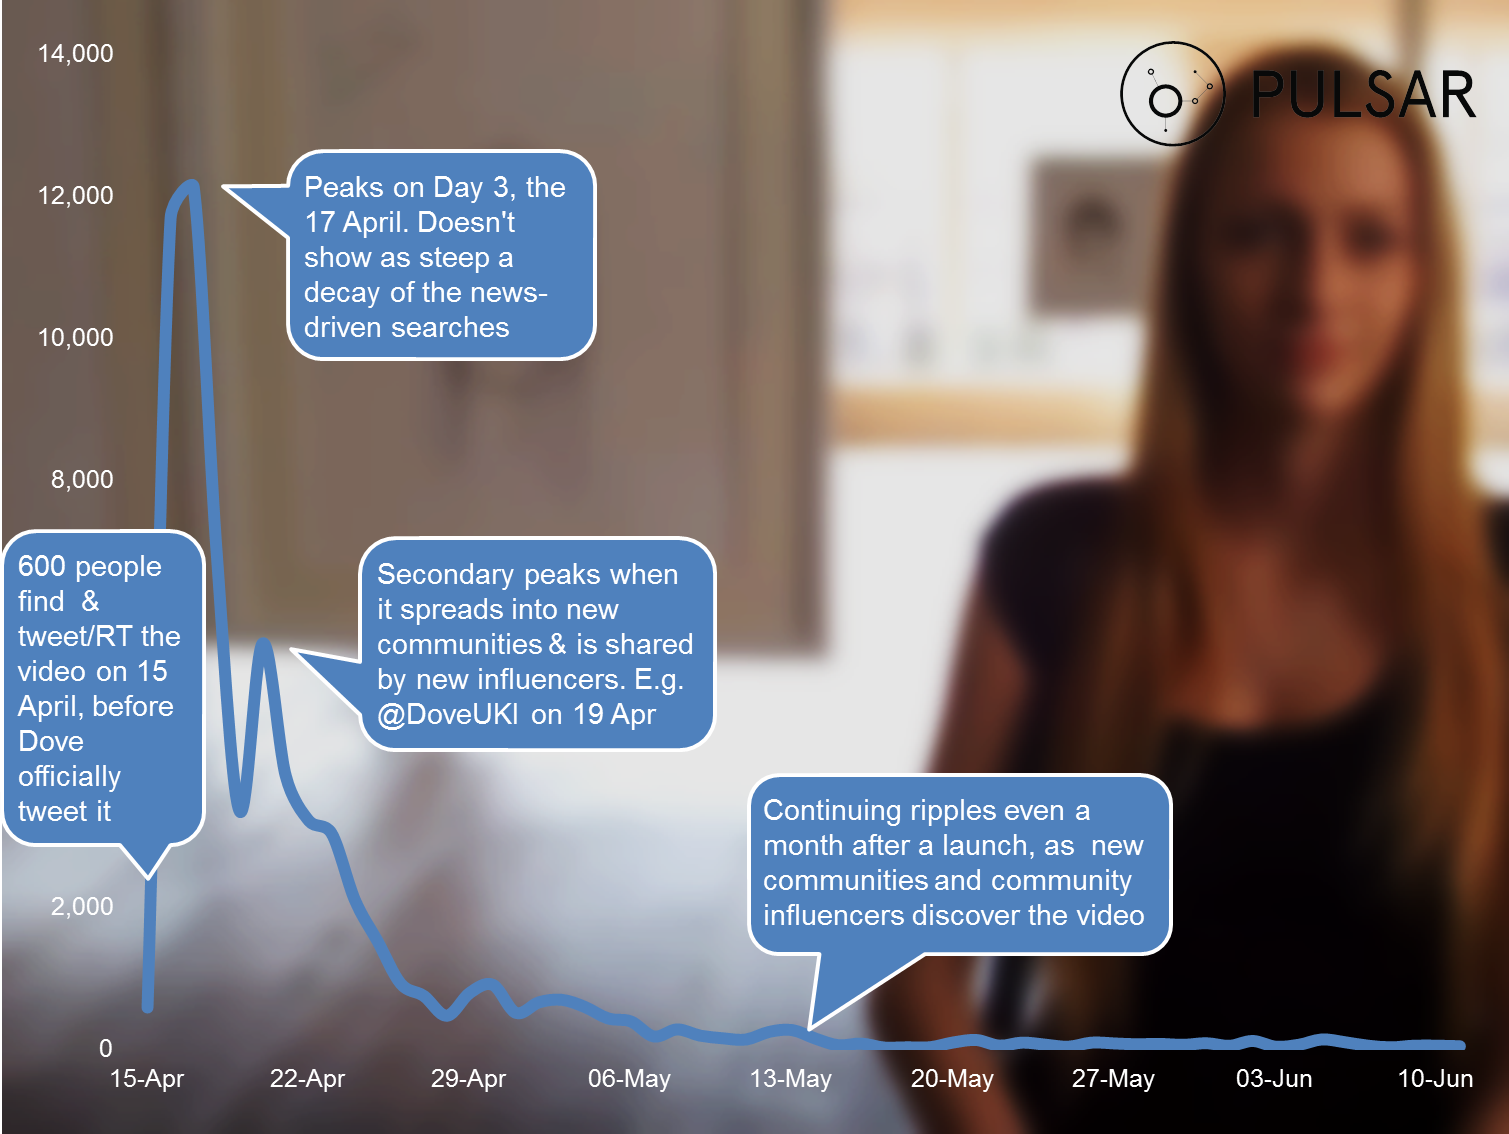
\includegraphics[width=120mm]{facegroup.png}
\caption{Graph from \emph{Facegroup} depicting the uptake of the "Dove Real Beauty Sketches" YouTube video, demonstrating the "spike" model as proposed by \emph{Facegroup}.\cite{facegroup}}
\label{sir}
\end{figure}
\newpage
Returning to an academic setting, Nika et al. recently undertook
another study to improve the fit of their real time fitting framework,
stating that, based on their previous study, a single epidemic is
inadequate to characterise a complex internet-based phenomena. This
may be because internet based trends may be influenced by multiple
underlying spreading mechanisms at different times, similar to the
`media effects' as described by Tweedle and Smith in their analysis of
`Bieber Fever'. Nika et al. took inspiration from Fourier analysis,
proposing that modelling and predicting internet-based phenomena could
be better described by considering multiple compartmental
epidemiological models. That is, an epidemic signal can be broken down
into a number of sub-epidemic models which, when recombined, can be
used as a predictive model (see Figure 1). Nika et al. go on to coin
the term \emph{synthedemic} from the field of syndemics - the idea
that infections can co-occur and interact with each other as well as
environmental factors. 

The term synthedemic is used to describe the co-occurence of a set of
infections, whether they are dependent or not. The aim of the study
was to account for the potential influence of multiple underlying
spreading mechanisms which may begin at different times by breaking an
incoming epidemic signal into component parts, and selecting the model
that best explains each component. Using only a classical SIR model
and exponential decay model as candidates, Nika et al. are able to
adequately characterise the evolution of synthetic data and four
real-world data sets from internet trends (BitTorrent downloads and
daily Youtube views) well. Please refer to Box 2 for a detailed
explanation of the theory used by Nika et al. Using synthetic double
epidemic data, the model by Nika et al. successfully predicts two
overlapping epidemics, predicting the peak of the second, spike
epidemic with a high RSquare value. The model is also fit successfully
to the BitTorrent downloads of two popular songs and a viral YouTube
video; detecting the presence of multiple outbreaks and exponential
decay of interest.
\newpage
\begin{framed}
{\begin{center}{\bf Box 2}\end{center}}
{\bf Methodology}:\\
The modelling procedure begins by considering a small, truncated
dataset of an epidemic outbreak. At each time point, an additional
data point is added until the end of the considered time frame is
reached. This might be a synthetic epidemic dataset, a historical
infectious disease epidemic, or some measure of interest in an online
phenomena (Nika et al. use BitTorrent downloads and daily YouTube
views). Nika et al. propose two candidate models that provide
theoretical analogues to the \emph{growth} and \emph{spike} trends as
proposed by \emph{Facegroup}: an SIR model to represent gradual
growth, and an exponential model to represent a rapid outbreak and
decay of public interest.\cite{facegroup}\\\\

At every time point, the multiple epidemic is optimised by attempting
to minimise the sum of squared error of the model against the data. At
each stage of fitting, the latest residuals are checked at each
additional time point for the presence of an additional epidemic
outbreak. If detected, a new epidemic is temporarily added to the
model from the list of candidate models. If the addition of this model
improves the $R^2$ value, then this additional epidemic is included in
all future model fittings. After the multiple epidemic model has been
optimised, an autoregressive model is fitted to capture the remaining
variability in the data. Finally, thefit of the multiple epidemic AR
model is assessed against benchmarked fitting procedures, such as a
single epidemic model, using a range of statistical tests, including
rSquare comparison.

{\bf Candidate Models}:\\
Let \emph{M} be the class of sub epidemic models under consideration: 

 \begin{equation*} M  = \{f_{1}^{(i)}, f_{2}^{(i)}\} \end{equation*}

Where $f_1^{(i)}$ and $f_2^{(i)}$ are defined as follows:
\begin{enumerate}[label=\Alph{*}.]
	\item $f_1^{(i)}$ denotes the SIR model $f_1^{(i)}(\theta^{(i)}, t)$ with parameter vector $\theta^{(i)} = [I_0^{(i)}, S_0^{(i)}, \beta^{(i)}, \gamma^{(i)}]$
\begin{equation*}
	\begin{split}
	&\frac{dS}{dt} = -\beta IS, \\
	&\frac{dI}{dt} = \beta IS - \gamma I, \\
	&\frac{dR}{dt} = \gamma I
	\end{split}
\end{equation*}
	\item $f_2^{(i)}$ denotes the Exponential decay model $f_2^{(i)}(\theta^{(i)}, t)$ with parameter vector $\theta^{(i)} = [I_0^{(i)}, \gamma^{(i)}]$
\begin{equation*}
	\frac{dI}{dt} = - \gamma I
\end{equation*}
\end{enumerate}
	
Parameter \emph{t} denotes a particular time, where $S_0^{(i)}$ and
$I_0^{(i)}$ denote the initial number of susceptible and infectious
individuals at time \emph{t}, whilst $\beta^{(i)}$ and
$\gamma^{(i)}$denote the infection and recovery rate. Furthermore, the
current number of sub epidemics within the overall model is given by
\emph{k}, where the combined value of the epidemic model at time
\emph{t} is given by the following formula:

\begin{equation*}
	\hat{y}(\theta ,t) = \sum\limits_{i=1}^k f^{(i)}(\theta^{(i)} ,t)
\end{equation*}
\end{framed}

Global mathematical models of epidemic processes provide a useful
insight into infectious disease dynamics; however, they make a number
of potentially unrealistic assumptions. Most notably, SIR models
assume complete mixing of the population. That is, each individual in
the population has an equal chance of coming into contact with every
other individual in the population. Although this assumption may hold
in certain scenarios (it is generally safe to assume that the internet
population observes random mixing), it may not be applicable to many
systems that are affected by local dynamics. Consider the population
of a town comprising of schools, offices and homes. Obviously a
student will mix much more frequently with other students and their
family rather than office workers. In such cases, the approach of SIR
based modelling may not be sufficient to capture the underlying
dynamics of the population. Many researchers have therefore developed
extended models to investigate stochasticity, multiple compartments
representing different subpopulations, branching processes and
chain-binomial models.\cite{computational}

One recent approach of particular relevance to the study of epidemic
phenomena in a social context is that of networked epidemiology: an
approach that encompasses individual behaviour, heterogenous
multiscale networks and the dynamical processes on these
networks. Although this particular project focuses on the application
of classical SIR modelling, it is worth discussing networked
epidemiology in brief to give a complete picture of the field.

\section{Networked Epidemiology and Social Networks} 

We have briefly touched on the idea of networks in epidemiology with
reference to multi-layered epidemic models, however it is worth
discussing the basics behind network considerations.\cite{tizzoni,
  gefm} Networked epidemiology takes its inspiration from graph
theory, using nodes to denote individuals and edges to denote
interactions. 

Let \emph{G(V,E)} denote a contact graph on a population of \emph{V}
individuals, where each edge, \emph{e = (u, v) $\in$ E} denotes those
individuals, \emph{u, v $\in$ V} that come into contact. As in the SIR
model, each node might be in the \emph{ S, I} or \emph{R}
state. However, the key difference is that the infection may only
spread from \emph{u} to \emph{v} along an edge with a probability of
$\beta$(\emph{e, t}) at time instant \emph{t} after \emph{u} has
become infected. Similarly, a node only remains infected for a set
amount of time denoted by $\tau$(\emph{u}). After this time, the node
\emph{u} switches to state $R$. By considering this network model over
a given number of time steps, the dynamics of an epidemic taking place
in a network can be modeled. With this basic idea, it is easy to see
how real world networks structures and data can be used to vastly
improve models of epidemic processes in reality, thereby improving
approaches to vaccination and disease control programmes.\cite{danon}
On the other hand, the reality of transmission networks is not quite
so ideal, with information regarding population connectivity and
interactions being limited. In this section, we will discuss a sample
of studies that build on the concept of local network approaches, and
discuss some approaches that have been taken towards applying these to
online trends.

With the basis for another approach to epidemic modelling, we can
begin to consider general frameworks to describe local dynamical
processes. One such approach is called the graphical discrete
dynamical system (GDDS)\cite{bisset}, which is defined as a tuple
(\emph{G, F, $\pi$)}), where: \emph{G = (V, E)} represents the
underlying contact network;  \emph{F = \{f\textsubscript{v}$|$v $\in$
  V\}} is a set of local functions for each node, \emph{v}, to compute
the state of \emph{v} based on its neighbours; and $\pi$ is a schedule
that specifies the order in which the stages of the nodes are
updated. It is possible to view the configuration space of a GDDS as a
Markov chain, \emph{M}, where each node in \emph{M} is the state
vector of the node states in the GDDS, \emph{G}. For example, in the
SIR model these three states correspond to the susceptible, infectious
and recovered states. 

A conceptually simpler approach to local network modelling is that of
a cellular automata model. Cellular automata models take into
consideration local behaviour and heterogeneity by ascribing each
individual to a particular cell as part of a grid. Individual cells
may have a certain state, such as infected or susceptible, and may
interact with other cells depending on the assumptions made. Turner et
al. provide one such example of this type of model, proposing two
spatial host-pathogen models that are described as equivalent to a
density and frequency dependent global model.\cite{turner} Another
example is provided by Zanette and Risau-Gusman, who investigate the
effect of evolving connections between individuals affects the spread
of an infection. Zanette and Risau-Gusman use an SIS based model where
susceptible agents are able to break their links with infected agents
either temporarily or permanentely, showing that a moderate contact
reconnection frequency is sufficient to suppress
infection.\cite{zanette}  It is possible to stretch the analogy of
human networks to the internet, with towns and cities representing
various internet communities. However, the drastically higher level of
connectivity and transmission speed on the internet does limit the
applicability of these locally driven models.

Global models may provide a more appropriate approach to global
internet trends compared to locally driven models; however, research
into using network based models to describe the dynamics of social
networks has recently shown some success. The aim of such models are
largely to predict future viral trends. One such example is a study by
Altshuler et al., who investigated the use of social diffusion models
in trend prediction in an online social trading
community.\cite{altshuler} Altshuler et al. set out to answer the
following question: given a snapshot of a social network with some
behaviour occurences, what is the probability that these occurences
will result in a viral diffusion and a wide-spread trend? The authors
model the diffusion process using scale-free networks (ie. probability
that \emph{v} has \emph{d} neighbours follows a power law); taking
into account local fluctuations and heterogeneity. From this,
Altshuler et al. develop a theoretical mathematical model to
understand trend diffusion in social networks. However, as the authors
points out, their framework needs to be tested in the field by
conducting an active experiment in which the emergence of a trend is
predicted in real time.

\section{Summary}
Research into the mathematical modelling of epidemic processes is now
an established field, with the majority of work based on the original
SIR model as proposed by Kermack and McKendrick.\cite{kermack}
Extensions of the SIR model take into account additional compartments
and inter-compartment dynamics, such as the inclusion of an `exposed'
group or of births and deaths. By customising model parameters and
structure, public health authorities and researchers can improve their
understanding of the way in which infectious diseases spread. For
example, using an SIS (infected individuals return to the susceptible
state) to model HIV, or an MSIR model (initial maternal-derived
immunity) in the case of measles.\cite{vynnycky} Understanding these
population dynamics in combination with the critical vaccination
threshold, given by the reproductive ratio of the virus, allows for
effective vaccination and control strategies. Particular topics of
note in recent years are the use of multi-layered epididemic models
and the use of maximum-likelihood estimations to predict the spread of
an epidemic in real time. \cite{tizzoni, gefm, white, hall, nishiura}

Although infectious diseases are the focus of mathematical modelling
of epidemic processes, a novel application is in the modelling of
internet-based phenomena and trends. As online social networks and
content sharing site become increasingly popular, the relevance of
understanding the dissemination of information online becomes an
increasingly important area of research both from an academic and
commercial perspective.\cite{cannarella, facebook} Studies in this
area are still at an early stage, though a few recent studies have
shown promising early results. \cite{marily2013, marily2014, bieber}
The study by Nika et al. shows promising results be considering the
presence of multiple, overlapping epidemics to describe one epidemic
phenomena in real time using a least-squares based fit. That is, the
popularity of a single online trend may be described through
considering its underlying sub-epidemic components. Nika et
al. consider two types of sub epidemic model as proposed by the
strategic insight agency, \emph{Facegroup}, and is the first study to
consider multiple overlapping epidemics to explain the spread of
internet trends. 

Although applying epidemic modelling techniques to the spread of
internet trends has shown promising results, there are a number of
limitations and flawed assumptions that must be considered. Firstly,
the analogy between an internet trend and an infectious disease is
limited. Nika et al. point out that whereas normal SIR modelling will
be able to make realistic assumptions or measurements regarding the
size of the initial susceptible population, this is not possible when
considering online trends. This $S_0$ value must therefore be treated
as an additional unknown parameter.\cite{marily2013} Furthermore, the
spreading mechanisms and lifecycle of internet trends are different to
those of infectious diseases. Whereas infectious diseases must be
passed on through physical contact, internet trends can be spread
instantaneously to any other user through a `tweet' or `share'. Trends
such as online videos or memes may also typically experience media
spikes when a video or celebrity is shown on television or highly
frequented web pages. The dangers of making such assumptions can be
observed in the study by Cannarella et al. who attempted to show that
Facebook would be abandoned by 2015, neglecting to consider that
Facebook will continue to `evolve' to keep users.\cite{cannarella,
  facebook} Proxies for interest in internet trends such as
\emph{Google Trends} search results should therefore be used with
caution.

Despite these limitations, promising early results encourage the
pursuit of further research. There are a number of other techniques
and models currently being investigated in infectious disease
modelling that might be applicable to the spread of internet
trends. For example, the use of maximum-likelihood estimations rather
than least squares;\cite{tizzoni} the use of multi-layered epidemic
models that might account for underlying social network structure (for
example, the spread of a viral video on or between social network
sites);\cite{altshuler, tizzoni} and the consideration of alternative
compartmental models or statistical distributions.\cite{meme}

With so many potential routes to follow, this project will focus on furthering the work done by Nika et al. to fit a multiple epidemic model in real time to the spread of online phenomena.

\section{Development Environment}
\subsection{Programming Languages}
There were a number of candidate programming languages, each with
their own strengths and weaknesses. In the end, R and C++ were chosen
for intitial and final implementations. Previous
approaches to epidemic and synthedemic model fitting frameworks use R
due to its readily available ODE solvers, optimisation functions and
graph plotting functionality.\cite{marily2013,marily2014} R therefore
provided an ideal means to implement the single and multiple epidemic
fitting frameworks initially. Once this initial model fitting
framework was implemented, we went on to provide a C++ implementation
with the aim of providing a faster, more transparent `from scratch'
fitting methodology.

At the start of the project, it was desirable to begin exploring and
understanding the theory behind epidemic modelling and otpimised model
fitting. As such, the first development consideration was to decide on
a language that was well adapted for easy implementations with a large
number of available packages and functions. R and Matlab were
candidates for this initial approach. Whilst Matlab has an arguably
better programming environment with better documentation, R has
already been shown to be effective in epidemic model fitting. The R
community provides a number of statistical analysis tools and is suited to dealing with non-typed data
sets, making it an ideal choice. These packages can easily be obtained
via the Comprehensive R Archive Network (CRAN).

The nature of parameter optimisation means that fitting a large number
of parameters simultaneously can be extremely slow, and an approach to
providing a faster implementation was to reimplement the model fitting
procedure in C++. C++ has been shown to be considerably faster than
both R and Matlab when solving stochastic neoclassical growth models,
suggesting that an efficient C++ implementation might provide a much
faster fitting framework than an R counterpart.\cite{languagespeed}
However, the trade off with run time speed is the fact that coding the
same algorithms and functions in C++ is very time consuming. Whilst
there are R packages readily available that allow parameter fit optimisation,
maximum likelihood estimations and graph plotting in only a few lines
of code, the equivalent functionality in C++ had to be implemented
from scratch. A significant challenge of this project was therefore to
find, adapt or create source code for the essential functions of the
model fitting framework. For graph plotting, a Gnuplot iostream was called from C++
code. 

Python and Java were also considered as potential languages for a
faster implementation. However, the relatively lower speed of Python and
unfamiliarity with Java meant that C++ remained the ideal choice.

It should be noted that whilst C++ provides an ideal way of speeding
up computational bottlenecks in the model fitting procedure (namely
the optimisation step), it it may still be desirable to call R
functions from within the C++ program. For example, the generation of
a likelihood profile. This can be achieved using the
Rcpp library if needed. Furthermore, the quick generation of synthetic
data with which to evaluate and develop the fitting framework is
clearly not a limiting factor. R therefore remained the ideal language
for syynthetic data generation using \emph{GillespieSSA} package,
exporting the data as a .csv file to be imported in the C++ implementation. 
